\documentclass{article}

\usepackage{amsmath}
\usepackage{graphicx}

\newcommand{\maxcut}{{\sc MaxCUT}}

\title{Quantum programming TP 2: QAOA for {\sc MaxCUT}}

\begin{document}
\maketitle
\begin{abstract}
This second TP is about the Quantum Approximate Optimization Algorithm (QAOA), which
is a quantum heuristic for combinatorial optimization problems.
We will work with the example of {\sc MaxCUT}, which consists in,
given a graph, figuring out how to partition its vertices into two
sets such that the number of edges having one end in each set is maximized.

QAOA is an hybrid ``quantum-classical'' algorithm, in which a the (continuous)
parameters of a quantum circuit are optimized by a \emph{classical} optimizer.
These parameters are typically angles of rotation gates in the circuit,
as we will see. The goal of the classical optimizer is to find the angles
that output a state which minimizes the \emph{cost function/Hamiltonian}
associated to the problem.

The jupyter notebook associated to this TP has to be completed
following the questions written below. You then have to send it
completed, by mail, to either bertrand.marchand@lix.polytechnique.fr
or bertrand.marchand7@gmail.com by \textbf{Friday January 6th 2023}.
It will be graded (common grade with the previous TP).

Besides sending a code implementing correct computation,
the clarity of the code and the presence of \emph{comments}
will be taken into account in the grading. The purpose on our side
is to assess how much you understood QAOA and the encoding
of MaxCUT onto a quantum computer.
\end{abstract}


\section{Question 1: Hamiltonian encoding {\sc MaxCUT}}

In the following, $G=(V,E)$ denotes a graph with vertex set $V$ and
edge set $E$.

\paragraph{Formal definition of \maxcut:}~\\
\textbf{Input:} a graph $G=(V,E)$\\
\textbf{Output:} a partition of $V$ into two sets $S$ and $V\setminus S$ such that $|\{(x,y)\in E\mid x\in S, y\in V\setminus S\}|$,
the number of ``cut'' edges is maximized.~\\

$S$ is then typically called a ``cut'' of the graph.

\paragraph{Physical interpretation} If you imagine that there is a $1/2$-spin (i.e. which can be ``up'' or ``down'') at 
each vertex of the graph, then the solution is the ground state of an Hamiltonian with pairwise anti-ferromagnetic 
interaction at each edge.

\paragraph{Encoding of \maxcut} With the vertices of $G$ numbered from $1$ to $n$,
a computational basis state\footnote{$\forall i x_i\in\{0,1\}$ and $|x\rangle=|x_1\rangle\otimes\dots\otimes|x_n\rangle$} 
$|x\rangle=|x_1\dots x_n\rangle$ will represent a cut $S=\{i\in V \mid x_i = 1\}$.

\paragraph{Question 1} Knowing that $\langle x | \sigma_z^k | x\rangle=\langle x | I\otimes \dots \otimes \underbrace{\sigma_z}_{\text{index }k} \otimes\dots \otimes I | x \rangle = (1-2x_k)$
and $\langle x | \otimes_{k=1}^n M_k | x \rangle = \prod_{k=1}^{n} \langle x_k | M_k |x_k \rangle$ 
(Some precisions: \footnote{With $M_k$ some 
2-by-2 matrix},\footnote{$\sigma_z=\begin{pmatrix}1 & 0 \\ 0 & -1\end{pmatrix}$}):\\~\\ 
Write down in latex in the notebook (in text cell and using `\$\$') an Hamiltonian involving only $\sigma_z$ 
and the edges $E$ of the input graph whose ground state is the solution to \maxcut on $G=(V,E)$.

\section{Question 2: brute-solving \maxcut (possible since we only look at small graphs) }

\paragraph{Question 2} In the notebook cell where a partial implementation of a brute force
computation of the solution to \maxcut is already written, write the computation of the
energy (Hamiltonian) value associated to a state $|x\rangle$. 

\section{Question 3, 4 \& 5: implement and run QAOA}

\paragraph{Variational quantum algorithms} The Quantum Approximate Optimization Algorithm~\cite{farhi2014quantum} is 
an example of a variational quantum algorithm, a family of hybrid quantum-classical algorithms with various potential
applications~\cite{cerezo2021variational}\footnote{including the chemisry problem you worked on last week}.

As depicted on Figure~\ref{qaoa}, QAOA consists of a quantum and a classical part. For the classical part, we will
use an optimizer from the Python package Scipy. The quantum part of QAOA consists of an initialization and a succession of $p$ \emph{layers}.
=
As described in \cite{farhi2014quantum}, one layer of QAOA consists of:
\begin{itemize}
    \item[1.] One rotation $RX(\theta)$ on each qubit, parameterized 
    by some angle $\theta$ common to all qubits. 
    \item[2.] A ``cost function'' layer in which the unitary evolution generated
    by the cost function Hamiltonian $e^{-i\beta H_{C}}$ is applied to the qubits. The parameter
    $\beta$ is the duration of the evolution.
    $$H_C = \sum_{i,j\in E} H_e(i,j)$$
    where the Hamiltonian $H_e(i,j)$ is a term representing edge $i,j$ which you have figured out in Question 1.
\end{itemize}

\paragraph{Question 3} Finish in the notebook the implementation of the function returning a QRoutine
for a qaoa layer, taking as input the set of edges, the number of qubits, $\theta$ and $\beta$. Use the $U_{ZZ}$ that is given.

\paragraph{Question 4} Complete the implementation of {\tt evaluate\_parameters} in the notebook. It takes as
input the number of qubits, the list of edges in the graph, the number of layers, and a vector of parameters.

The vector of parameters looks like $[\theta_1, \beta_1, \theta_2, \beta_2,\dots]$. The parameters $(\theta_i,\beta_i)$ for 
$1\leq i \leq p$ (i.e. one pair per layer) are all concatenated.


The initialization consists of a layer of Hadamard gates ($H$), one for each qubit.
Then, the parameterized circuit should use the qaoa layer routine you implemented in Question $3$.
Finally, you must compute the value of the observable on the state vector. A loop on the state of the state vector
is already given.

\begin{figure}

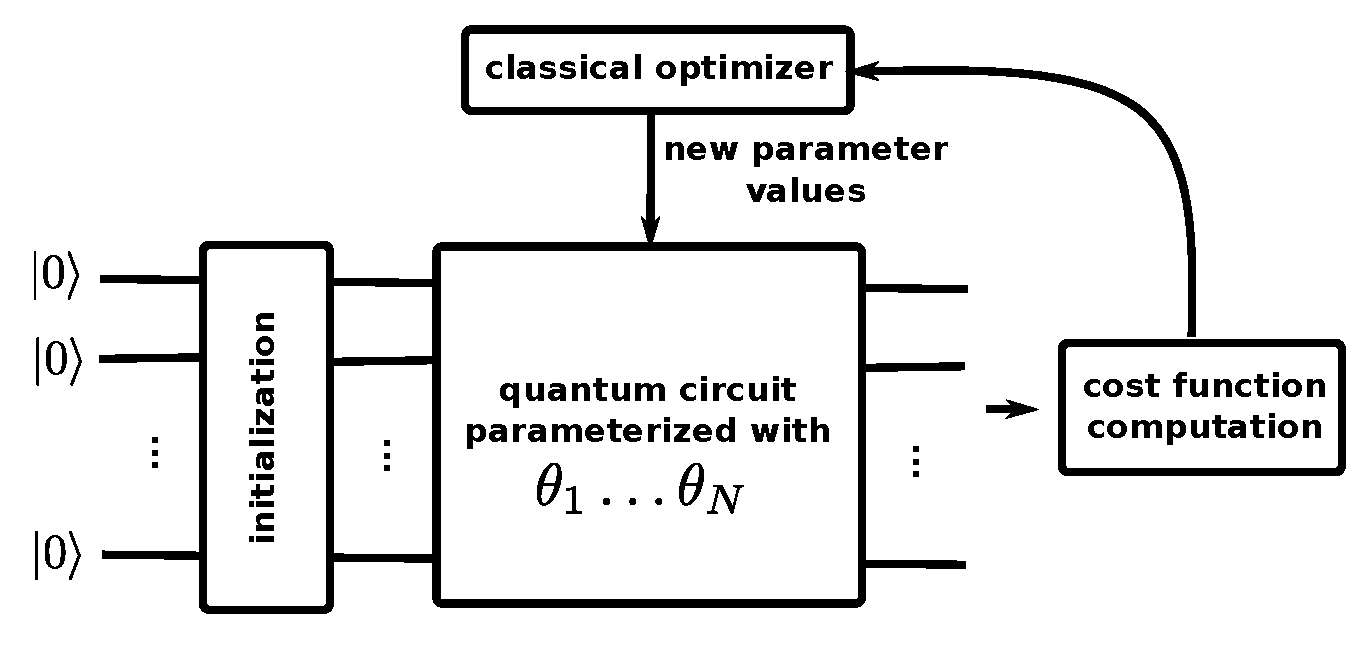
\includegraphics[width=\textwidth]{qaoa.pdf}

\caption{In our case, the ``initialization'' is simply a layer of Hadarmard gates, the parameterized circuit is a succession
    of $p$ QAOA layers, whose implementation is the subject of Question 3, and the goal of the optimizer is
    to find parameters that minimize the value of the ``cost function'' (i.e. the \maxcut  Hamiltonian) for the output
    quantum state of the circuit.}
\label{qaoa}
\end{figure}

\paragraph{Question 5} The remainder of the algorithm, with the classical optimizer, has been already implemented. Use it
to answer the following question: What number of layers is needed for QAOA to reach the optimum value 
for {\tt graph6} (choose the graph at the beginning of the notebook) ? Write the answer in the text cell with ``Question 5''.

\section{Smart initialization of parameters: Question 6}

The code run at Question 5 initializes the parameter vector with random values. Here we implement a better strategy.

\paragraph{Adiabatic Quantum Computing} QAOA is in fact linked to a flavour of quantum computing called Adiabatic 
Quantum Computing~\cite{albash2018adiabatic}. In AQC, the ground state of the Hamiltonian containing the answer to the problem
is reached through a slow transition from a simpler Hamiltonian (such as $\sum_k \sigma_x^k$) whose
ground state is easy to prepare ($\otimes_{k=1}^n\left(\frac{|0\rangle+|1\rangle}{\sqrt{2}}\right)$ for $\sum_k \sigma_x^k$)

The transition can consist for instance in going from $s=0$ to $T$ in $$ H(s) = (1-\frac{s}{T})\sum_k \sigma_x^k + \frac{s}{T} H_C $$

With $\sigma_x = \begin{pmatrix} 0 & 1\\ 1 & 0 \end{pmatrix}$.
The Adiabatic Theorem then states that if the transition is slow enough, the state at the end of the transition is the
ground state of $H_C$.

Integrating the Schr\"{o}dinger equation for this transition, we get:

$$ |\psi_{final}\rangle = e^{-i\int_0^T H(s)ds }|\psi_0\rangle $$

\paragraph{Quetion 6} Approximating the integral by $\int_0^T H(s)ds = \sum_{k=1}^p H(\frac{k}{p}\times T)\frac{T}{p}$ 
and supposing we are in conditions where $e^{A+B}\simeq e^A\cdot e^B$, Figure out theoretical optimal values for each $\theta_k,\beta_k$
of the parameter vector in QAOA\footnote{Note that for the initialization, the first layer of Hadamard does send $|0\rangle$
to $\frac{|0\rangle+|1\rangle}{\sqrt{2}}$}.

Implement that assignment of initial values in the notebook. What effect does it have on convergence ? You may try different values
of big $T$. 

A reference on this initialization technique:~\cite{sack2021quantum} 

\bibliography{biblio}
\bibliographystyle{unsrt}
\end{document}
